	%%%%%%%%%%%%%%%%%%%%%%%%%%%%%%%%%%%%%%%%%%%%%%%%%%%%%%%%%%%%%%%%
%
%  Template for homework of Introduction to Machine Learning.
%
%  Fill in your name, lecture number, lecture date and body
%  of homework as indicated below.
%         
%%%%%%%%%%%%%%%%%%%%%%%%%%%%%%%%%%%%%%%%%%%%%%%%%%%%%%%%%%%%%%%%
\documentclass[11pt,letter,notitlepage]{article}
%Mise en page
\usepackage[left=2cm, right=2cm, lines=45, top=0.8in, bottom=0.7in]{geometry}
\usepackage{fancyhdr}
\usepackage{fancybox}
\usepackage{graphicx}
\usepackage{pdfpages}
\usepackage{enumitem}
\usepackage{algorithm}
\usepackage{algorithmic}
\usepackage{pifont}
\renewcommand{\headrulewidth}{1.5pt}
\renewcommand{\footrulewidth}{1.5pt}
\newcommand\Loadedframemethod{TikZ}
\usepackage[framemethod=\Loadedframemethod]{mdframed}
\usepackage{amssymb,amsmath}
\usepackage{extarrows}
\usepackage{amsthm}
\usepackage{thmtools}
\usepackage{bm}
\usepackage{listings}
\usepackage{xcolor}
\usepackage{float}

\lstset{
    language=Python,
    basicstyle=\ttfamily\small,
    keywordstyle=\color{blue},
    commentstyle=\color{teal},
    stringstyle=\color{red},
    showstringspaces=false,
    breaklines=true,
    frame=single
}

\setlength{\topmargin}{0pt}
\setlength{\textheight}{9in}
\setlength{\headheight}{0pt}
\setlength{\oddsidemargin}{0.25in}
\setlength{\textwidth}{6in}
%%%%%%%%%%%%%%%%%%%%%%%%
%%%%%% Define math operator %%%%%
%%%%%%%%%%%%%%%%%%%%%%%%
\DeclareMathOperator*{\argmin}{\bf argmin}
\DeclareMathOperator*{\relint}{\bf relint\,}
\DeclareMathOperator*{\dom}{\bf dom\,}
\DeclareMathOperator*{\intp}{\bf int\,}
\DeclareMathOperator*{\minimize}{\bf minimize}
%%%%%%%%%%%%%%%%%%%%%%%
\setlength{\topmargin}{0pt}
\setlength{\textheight}{9in}
\setlength{\headheight}{0pt}
\setlength{\oddsidemargin}{0.25in}
\setlength{\textwidth}{6in}
\pagestyle{fancy}
%%%%%%%%%%%%%%%%%%%%%%%%
%% Define the Exercise environment %%
%%%%%%%%%%%%%%%%%%%%%%%%
\mdtheorem[
topline=false,
rightline=false,
leftline=false,
bottomline=false,
leftmargin=-10,
rightmargin=-10
]{exercise}{\textbf{Exercise}}
\renewcommand{\theexercise}{\arabic{exercise}:}
%%%%%%%%%%%%%%%%%%%%%%%
%% End of the Exercise environment %%
%%%%%%%%%%%%%%%%%%%%%%%
%%%%%%%%%%%%%%%%%%%%%%%%
%% Define the Problem environment %%
%%%%%%%%%%%%%%%%%%%%%%%%
\mdtheorem[
topline=false,
rightline=false,
leftline=false,
bottomline=false,
leftmargin=-10,
rightmargin=-10
]{problem}{\textbf{Problem}}
%%%%%%%%%%%%%%%%%%%%%%%
%% End of the Exercise environment %%
%%%%%%%%%%%%%%%%%%%%%%%
%%%%%%%%%%%%%%%%%%%%%%%
%% Define the Solution Environment %%
%%%%%%%%%%%%%%%%%%%%%%%
\declaretheoremstyle
[
spaceabove=0pt,
spacebelow=0pt,
headfont=\normalfont\bfseries,
notefont=\mdseries,
notebraces={(}{)},
headpunct={:},
headindent={},
postheadspace=\newline,
bodyfont=\normalfont,
qed=$\blacksquare$,
preheadhook={\begin{mdframed}[style=myframedstyle]},
postfoothook=\end{mdframed},
]{mystyle}
\declaretheorem[style=mystyle,title=Solution]{solution}
\mdfdefinestyle{myframedstyle}{%
	topline=false,
	rightline=false,
	leftline=false,
	bottomline=false,
	skipabove=-6ex,
	leftmargin=-10,
	rightmargin=-10,
	backgroundcolor=black!5}
%%%%%%%%%%%%%%%%%%%%%%%
%% End of the Solution environment

\renewcommand{\eqref}[1]{Eq.~(\ref{#1})}
\newcommand{\figref}[1]{Fig.~\ref{#1}}


\newcommand{\proj}[2]{\textbf{P}_{#2} (#1)}
\newcommand{\lspan}[1]{\textbf{span}  (#1)  }
\newcommand{\rank}[1]{ \textbf{rank}  (#1)  }
\newcommand{\tr}{ \operatorname{tr}  }
\newcommand{\RNum}[1]{\uppercase\expandafter{\romannumeral #1\relax}}

\newcommand{\mb}[1]{\mathbf{#1}}

\DeclareMathOperator*{\cl}{\bf cl\,}
\DeclareMathOperator*{\bd}{\bf bd\,}
\DeclareMathOperator*{\conv}{\bf conv\,}
\DeclareMathOperator*{\epi}{\bf epi\,}

% Definition environment	
\theoremstyle{definition}	
\newtheorem{definition}{Definition}	


%%%%%%%%%%%%%%%%%%%%%%%%%%%%%%%%%%%%%%%%%%
%%           Homework info.             %%
\newcommand{\posted}{\text{Apr. 13th, 2025}}       			%%% FILL IN POST DATE HERE
\newcommand{\due}{\text{May. 2nd, 2025}} 			%%% FILL IN Due DATE HERE
\newcommand{\hwno}{\text{4}} 		           			%%% FILL IN LECTURE NUMBER HERE
%%%%%%%%%%%%%%%%%%%%%%%%%%%%%%%%%%%%%%%%%%

%%%%%%%%%%%%%%%%%%%%%%%%%%%%%%%%%%%%
%%    Put your information here   %%
\newcommand{\name}{\text{Jinghao Chen}}  	          			%%% FILL IN YOUR NAME HERE
\newcommand{\id}{\text{PB23010359}}		       			%%% FILL IN YOUR ID HERE
%%%%%%%%%%%%%%%%%%%%%%%%%%%%%%%%%%%%

\lhead{
 	\textbf{\name}
}
\rhead{
 	\textbf{\id}
}
\chead{\textbf{
		Homework \hwno
}}


\begin{document}
	\vspace*{-4\baselineskip}
	\thispagestyle{empty}
	
	
	\begin{center}
		{\bf\large Introduction to Optimization}\\
		{Spring 2026}\\
		University of Science and Technology of China
	\end{center}
	
	\noindent
	Lecturer: Nick  			 %%% FILL IN LECTURER HERE
	\hfill
	Homework \hwno             			
	\\
	Posted: \posted
	\hfill
	Due: \due
    \\
	Name: \name             			
	\hfill
	ID: \id
	
	\noindent
	\rule{\textwidth}{2pt}
	
	\medskip
	
	
	
	
	
	%%%%%%%%%%%%%%%%%%%%%%%%%%%%%%%%%%%%%%%%%%%%%%%%%%%%%%%%%%%%%%%%
	%% BODY OF HOMEWORK GOES HERE
	%%%%%%%%%%%%%%%%%%%%%%%%%%%%%%%%%%%%%%%%%%%%%%%%%%%%%%%%%%%%%%%%

\begin{exercise}
Let $f$ be a differentiable function with $\operatorname{dom} f = \mathbb{R}^n$.

\begin{enumerate}[label=(\alph*)]
    \item If $\nabla f$ is Lipschitz continuous with parameter $L > 0$, show that
    \[
    g(x) := \frac{L}{2}\|x\|_2^2 - f(x)
    \]
    is convex. In addition, if $x^\star$ is a minimizer of $f$, show that
    \[
    \frac{1}{2L}\|\nabla f(x)\|_2^2 \le f(x) - p^\star \le \frac{L}{2}\|x - x^\star\|_2^2,
    \qquad \forall x.
    \]

    \item If $f$ is strongly convex with parameter $m > 0$, show that if there is a minimizer $x^\star$, it is unique and it holds that
    \[
    \frac{m}{2}\|x - x^\star\|_2^2 \le f(x) - p^\star \le \frac{1}{2m}\|\nabla f(x)\|_2^2,
    \qquad \forall x.
    \]

    \item Explain the implications of (a), (b) for optimization algorithms.

    \item If $f$ satisfies the assumptions of both (a) and (b), show that
    \[
    (\nabla f(y) - \nabla f(x))^T (y - x)
    \ge
    \frac{mL}{m+L}\|y-x\|_2^2
    +
    \frac{1}{m+L}\|\nabla f(y)-\nabla f(x)\|_2^2,
    \qquad \forall x,y.
    \]

    \textit{[Hint: The function}
    \[
    g := f - \frac{m}{2}\|\cdot\|_2^2
    \]
    \textit{is convex and $\nabla g$ is Lipschitz continuous with parameter $L-m$. This implies that}
    \[
    (\nabla g(y)-\nabla g(x))^T (y-x)
    \ge
    \frac{1}{L-m}\|\nabla g(y)-\nabla g(x)\|_2^2,
    \qquad \forall x,y. \textit{]}
    \]
\end{enumerate}
\end{exercise}

\newpage

\begin{solution}
Let $p^\star=f(x^\star)$.

\begin{enumerate}[label=(\alph*)]
    \item Since $\nabla f$ is $L$-Lipschitz, we have the standard quadratic upper bound
    \[
    f(y)\le f(x)+\nabla f(x)^T(y-x)+\frac{L}{2}\|y-x\|_2^2,
    \qquad \forall x,y.
    \]
    Define
    \[
    g(x)=\frac{L}{2}\|x\|_2^2-f(x).
    \]
    Then
    \[
    \nabla g(x)=Lx-\nabla f(x),
    \]
    and
    \[
    \begin{aligned}
    g(y)-g(x)-\nabla g(x)^T(y-x)
    &=\frac{L}{2}\|y\|_2^2-f(y)-\frac{L}{2}\|x\|_2^2+f(x)-(Lx-\nabla f(x))^T(y-x)\\
    &=\frac{L}{2}\|y-x\|_2^2-\Big(f(y)-f(x)-\nabla f(x)^T(y-x)\Big)\ge 0.
    \end{aligned}
    \]
    Hence $g$ is convex.

    Now let $x^\star$ be a minimizer of $f$. Since $f$ is differentiable on $\mathbb R^n$,
    \[
    \nabla f(x^\star)=0.
    \]

    Using the quadratic upper bound with base point $x^\star$,
    \[
    f(x)\le f(x^\star)+\nabla f(x^\star)^T(x-x^\star)+\frac{L}{2}\|x-x^\star\|_2^2
    =p^\star+\frac{L}{2}\|x-x^\star\|_2^2,
    \]
    so
    \[
    f(x)-p^\star\le \frac{L}{2}\|x-x^\star\|_2^2.
    \]

    For the other inequality, choose
    \[
    y=x-\frac1L\nabla f(x).
    \]
    Then
    \[
    \begin{aligned}
    f(y)
    &\le f(x)+\nabla f(x)^T\left(-\frac1L\nabla f(x)\right)
    +\frac{L}{2}\left\|-\frac1L\nabla f(x)\right\|_2^2\\
    &=f(x)-\frac1L\|\nabla f(x)\|_2^2+\frac1{2L}\|\nabla f(x)\|_2^2\\
    &=f(x)-\frac1{2L}\|\nabla f(x)\|_2^2.
    \end{aligned}
    \]
    Since $p^\star\le f(y)$,
    \[
    \frac1{2L}\|\nabla f(x)\|_2^2\le f(x)-p^\star.
    \]

    Therefore,
    \[
    \frac{1}{2L}\|\nabla f(x)\|_2^2 \le f(x)-p^\star \le \frac{L}{2}\|x-x^\star\|_2^2,
    \qquad \forall x.
    \]

    \item Since $f$ is strongly convex with parameter $m>0$,
    \[
    f(y)\ge f(x)+\nabla f(x)^T(y-x)+\frac{m}{2}\|y-x\|_2^2,
    \qquad \forall x,y.
    \]

    We first show uniqueness of the minimizer:
    
    $\forall$ $x$, $y$ $\in$ $\mathbb{R}^n$, $\theta\in (0,1)$, let $z=\theta x + (1-\theta)y$. By strong convexity,
    \[
    \left\{
    \begin{aligned}
    f(x) \geq f(z) + \nabla f(z)^T(x-z) + \frac{m}{2}\|x-z\|_2^2,\\
    f(y) \geq f(z) + \nabla f(z)^T(y-z) + \frac{m}{2}\|y-z\|_2^2,
    \end{aligned}
    \right.
    \]
    \[
    \begin{aligned}
    \implies
    &\theta f(x) + (1-\theta) f(y)\\
    \geq
    &f(z) + \nabla f(z)^{T} (\theta(x-z) + (1-\theta)(y-z)) + \frac{m}{2} \left( \theta \|x-z\|_2^2 + (1-\theta) \|y-z\|_2^2 \right)\\
    =
    &f(z) + \frac{m}{2}\theta(1-\theta)\|x-y\|_2^2.
    \end{aligned}
    \]
    \[
    \xLongrightarrow{m > 0}
    \theta f(x) + (1-\theta) f(y) > f(\theta x + (1-\theta) y)
    \]
    Hence $f$ is strictly convex, and the minimizer is unique.

    Since $x^\star$ is a minimizer and $f$ is differentiable,
    \[
    \nabla f(x^\star)=0.
    \]
    Applying strong convexity with $x=x^\star$ gives
    \[
    f(x)\ge f(x^\star)+\nabla f(x^\star)^T(x-x^\star)+\frac{m}{2}\|x-x^\star\|_2^2
    =p^\star+\frac{m}{2}\|x-x^\star\|_2^2,
    \]
    hence
    \[
    \frac{m}{2}\|x-x^\star\|_2^2\le f(x)-p^\star.
    \]

    For the upper bound, from strong convexity we have for every $y$,
    \[
    f(y)\ge f(x)+\nabla f(x)^T(y-x)+\frac{m}{2}\|y-x\|_2^2.
    \]
    Taking the infimum over $y$ yields
    \[
    p^\star\ge \inf_y \left\{ f(x)+\nabla f(x)^T(y-x)+\frac{m}{2}\|y-x\|_2^2 \right\}.
    \]
    The right-hand side is minimized at
    \[
    y=x-\frac1m\nabla f(x),
    \]
    and the minimum value equals
    \[
    f(x)-\frac1{2m}\|\nabla f(x)\|_2^2.
    \]
    Therefore
    \[
    p^\star\ge f(x)-\frac1{2m}\|\nabla f(x)\|_2^2,
    \]
    i.e.
    \[
    f(x)-p^\star\le \frac1{2m}\|\nabla f(x)\|_2^2.
    \]

    Hence
    \[
    \frac{m}{2}\|x-x^\star\|_2^2 \le f(x)-p^\star \le \frac{1}{2m}\|\nabla f(x)\|_2^2,
    \qquad \forall x.
    \]

    \item The inequalities in (a) and (b) provide error bounds relating three quantities:
    \[
    f(x)-p^\star,\qquad \|x-x^\star\|_2,\qquad \|\nabla f(x)\|_2.
    \]
    In particular:
    \begin{itemize}
        \item If $f$ is $L$-smooth, then small gradient implies small suboptimality:
        \[
        \frac1{2L}\|\nabla f(x)\|_2^2\le f(x)-p^\star.
        \]
        Also, closeness to $x^\star$ implies small objective error:
        \[
        f(x)-p^\star\le \frac{L}{2}\|x-x^\star\|_2^2.
        \]
        \item If $f$ is $m$-strongly convex, then objective error controls distance to the optimizer:
        \[
        \frac{m}{2}\|x-x^\star\|_2^2\le f(x)-p^\star,
        \]
        and gradient controls objective error:
        \[
        f(x)-p^\star\le \frac1{2m}\|\nabla f(x)\|_2^2.
        \]
    \end{itemize}
    Thus, in the strongly convex case, function error, gradient norm, and distance to the optimizer are all equivalent up to constants. This explains why gradient-based stopping criteria are meaningful, and why first-order methods behave much better in the strongly convex case.

    If both assumptions hold, then combining (a) and (b) gives
    \[
    2m\bigl(f(x)-p^\star\bigr)\le \|\nabla f(x)\|_2^2\le 2L\bigl(f(x)-p^\star\bigr),
    \]
    which is a fundamental basis for linear convergence results of gradient descent. The convergence speed depends on the condition number $\kappa=L/m$.

    \item Define
    \[
    h(x):=f(x)-\frac{m}{2}\|x\|_2^2.
    \]
    By strong convexity of $f$, $h$ is convex. By the hint, $\nabla h$ is Lipschitz continuous with parameter $L-m$, and
    \[
    (\nabla h(y)-\nabla h(x))^T(y-x)
    \ge
    \frac{1}{L-m}\|\nabla h(y)-\nabla h(x)\|_2^2.
    \]

    Let
    \[
    \Delta x := y-x,\qquad \Delta \nabla := \nabla f(y)-\nabla f(x).
    \]
    Since
    \[
    \nabla h(y)-\nabla h(x)=\Delta \nabla - m\Delta x,
    \]
    the above inequality becomes
    \[
    (\Delta \nabla-m\Delta x)^T\Delta x
    \ge
    \frac{1}{L-m}\|\Delta \nabla-m\Delta x\|_2^2.
    \]
    Expanding both sides,
    \[
    \Delta \nabla^T\Delta x-m\|\Delta x\|_2^2
    \ge
    \frac{1}{L-m}
    \left(
    \|\Delta \nabla\|_2^2-2m\,\Delta \nabla^T\Delta x+m^2\|\Delta x\|_2^2
    \right).
    \]
    Multiply by $L-m$:
    \[
    (L-m)\Delta \nabla^T\Delta x-m(L-m)\|\Delta x\|_2^2
    \ge
    \|\Delta \nabla\|_2^2-2m\,\Delta \nabla^T\Delta x+m^2\|\Delta x\|_2^2.
    \]
    Rearranging,
    \[
    (L+m)\Delta \nabla^T\Delta x
    \ge
    \|\Delta \nabla\|_2^2+mL\|\Delta x\|_2^2.
    \]
    Therefore
    \[
    \Delta \nabla^T\Delta x
    \ge
    \frac{mL}{m+L}\|\Delta x\|_2^2
    +
    \frac{1}{m+L}\|\Delta \nabla\|_2^2.
    \]
    Replacing $\Delta x,\Delta \nabla$ by their definitions,
    \[
    (\nabla f(y)-\nabla f(x))^T(y-x)
    \ge
    \frac{mL}{m+L}\|y-x\|_2^2
    +
    \frac{1}{m+L}\|\nabla f(y)-\nabla f(x)\|_2^2.
    \]
\end{enumerate}
\end{solution}

\newpage

\begin{exercise}
Analyze the gradient descent method for each of the following cases.

\begin{enumerate}[label=(\alph*)]
    \item $f$ has $L$-Lipschitz gradient. Show that
    \[
    f(x^{(k)}) - f(x^{(k-1)})
    \le
    -t^{(k)}
    \left(1 - \frac{L t^{(k)}}{2}\right)
    \|\nabla f(x^{(k-1)})\|_2^2,
    \]
    therefore for $t^{(k)} \in \left(0,\frac{2}{L}\right)$ GD is a descent method.

    \textit{[Hint: Use the quadratic upper bound (Hw1, problem 6a):}

Let $f$ be a differentiable function with $\operatorname{dom} f = \mathbb{R}^n$.

\begin{enumerate}[label=(\alph*)]
    \item If there exists $L \ge 0$ such that
    \[
    \|\nabla f(y)-\nabla f(x)\|_2 \le L\|y-x\|_2,
    \qquad \forall x,y,
    \]
    show that
    \[
    f(y) \le f(x)+\nabla f(x)^T(y-x)+\frac{L}{2}\|y-x\|_2^2,
    \qquad \forall x,y.
    \]

    \textit{[Hint: Use that
    $
    f(y)=f(x)+\int_0^1 \nabla f\bigl(x+t(y-x)\bigr)^T (y-x)\,dt.
    $]]}
\end{enumerate}

    \item In addition to the assumption in (a), $f$ is lower-bounded. For fixed step-size $t=\frac{1}{L}$, show that
    \[
    \min_{i=0,\ldots,k} \|\nabla f(x^{(i)})\|_2^2
    \le
    \frac{2L}{k+1}\bigl(f(x^{(0)}) - p^\star\bigr).
    \]

    \item In addition to the assumptions in (b), $f$ is convex and attains the minimum at $x^\star$. Show that
    \[
    f(x^{(k)}) - p^\star
    \le
    \frac{L}{2k}\|x^{(0)} - x^\star\|_2^2.
    \]

    \item In addition to the assumptions in (c), $f$ is strongly convex with parameter $m>0$. Show that for fixed step-size
    \[
    t \in \left(0,\frac{2}{m+L}\right)
    \]
    it holds that
    \[
    \|x^{(k)} - x^\star\|_2^2
    \le
    \rho^k \|x^{(0)} - x^\star\|_2^2,
    \qquad
    \rho := \left(1 - t\frac{2mL}{m+L}\right).
    \]

    \textit{[Hint: Use the bound from problem 1d]}

    For the value of $t$ that minimizes the upper bound, express $\rho$ as a function of the condition number
    \[
    \kappa := \frac{L}{m},
    \]
    and also derive a bound for $f(x^{(k)}) - p^\star$ as a function of $f(x^{(0)}) - p^\star$.

    \item Explain the implications of parts (b) (for non-convex optimization) and parts (c), (d) for convex optimization by analyzing the number of iterations needed to attain a given accuracy $\epsilon$.
\end{enumerate}
\end{exercise}

\newpage

\begin{solution}
Let the GD iteration be
\[
x^{(k)}=x^{(k-1)}-t^{(k)}\nabla f(x^{(k-1)}).
\]

\begin{enumerate}[label=(\alph*)]
    \item Since $\nabla f$ is $L$-Lipschitz, we have the quadratic upper bound
    \[
    f(y)\le f(x)+\nabla f(x)^T(y-x)+\frac{L}{2}\|y-x\|_2^2,
    \qquad \forall x,y.
    \]
    Apply this with
    \[
    x=x^{(k-1)},\qquad y=x^{(k)}=x^{(k-1)}-t^{(k)}\nabla f(x^{(k-1)}).
    \]
    Then
    \[
    y-x=-t^{(k)}\nabla f(x^{(k-1)}),
    \]
    hence
    \[
    \begin{aligned}
    f(x^{(k)})
    &\le
    f(x^{(k-1)})
    +\nabla f(x^{(k-1)})^T\bigl(-t^{(k)}\nabla f(x^{(k-1)})\bigr)
    +\frac{L}{2}\left\|-t^{(k)}\nabla f(x^{(k-1)})\right\|_2^2\\
    &=
    f(x^{(k-1)})
    -t^{(k)}\|\nabla f(x^{(k-1)})\|_2^2
    +\frac{L(t^{(k)})^2}{2}\|\nabla f(x^{(k-1)})\|_2^2.
    \end{aligned}
    \]
    Therefore
    \[
    f(x^{(k)}) - f(x^{(k-1)})
    \le
    -t^{(k)}
    \left(1 - \frac{L t^{(k)}}{2}\right)
    \|\nabla f(x^{(k-1)})\|_2^2.
    \]
    If
    \[
    t^{(k)}\in\left(0,\frac{2}{L}\right),
    \]
    then $1-\frac{Lt^{(k)}}2>0$, so GD is a descent method.

    \item Now fix $t=\frac1L$. Then from part (a),
    \[
    f(x^{(k+1)})-f(x^{(k)})
    \le
    -\frac1L\left(1-\frac12\right)\|\nabla f(x^{(k)})\|_2^2
    =
    -\frac1{2L}\|\nabla f(x^{(k)})\|_2^2.
    \]
    Hence
    \[
    \frac1{2L}\|\nabla f(x^{(k)})\|_2^2
    \le
    f(x^{(k)})-f(x^{(k+1)}).
    \]
    Summing from $i=0$ to $k$ gives
    \[
    \frac1{2L}\sum_{i=0}^k \|\nabla f(x^{(i)})\|_2^2
    \le
    f(x^{(0)})-f(x^{(k+1)}).
    \]
    Since $f$ is lower bounded and $p^\star=\inf f$,
    \[
    f(x^{(k+1)})\ge p^\star,
    \]
    so
    \[
    \sum_{i=0}^k \|\nabla f(x^{(i)})\|_2^2
    \le
    2L\bigl(f(x^{(0)})-p^\star\bigr).
    \]
    Therefore
    \[
    \min_{i=0,\ldots,k}\|\nabla f(x^{(i)})\|_2^2
    \le
    \frac1{k+1}\sum_{i=0}^k \|\nabla f(x^{(i)})\|_2^2
    \le
    \frac{2L}{k+1}\bigl(f(x^{(0)})-p^\star\bigr).
    \]

    \item Assume in addition that $f$ is convex and attains its minimum at $x^\star$. We still use the fixed step-size $t=\frac1L$.

    First, from
    \[
    x^{(k+1)}=x^{(k)}-\frac1L\nabla f(x^{(k)}),
    \]
    we have
    \[
    \begin{aligned}
    \|x^{(k+1)}-x^\star\|_2^2
    &=
    \left\|x^{(k)}-x^\star-\frac1L\nabla f(x^{(k)})\right\|_2^2\\
    &=
    \|x^{(k)}-x^\star\|_2^2
    -\frac{2}{L}\nabla f(x^{(k)})^T(x^{(k)}-x^\star)
    +\frac1{L^2}\|\nabla f(x^{(k)})\|_2^2.
    \end{aligned}
    \]
    Rearranging,
    \[
    \nabla f(x^{(k)})^T(x^{(k)}-x^\star)
    =
    \frac L2\Bigl(\|x^{(k)}-x^\star\|_2^2-\|x^{(k+1)}-x^\star\|_2^2\Bigr)
    +\frac1{2L}\|\nabla f(x^{(k)})\|_2^2.
    \]
    By convexity,
    \[
    f(x^{(k)})-p^\star
    =
    f(x^{(k)})-f(x^\star)
    \le
    \nabla f(x^{(k)})^T(x^{(k)}-x^\star).
    \]
    Hence
    \[
    f(x^{(k)})-p^\star
    \le
    \frac L2\Bigl(\|x^{(k)}-x^\star\|_2^2-\|x^{(k+1)}-x^\star\|_2^2\Bigr)
    +\frac1{2L}\|\nabla f(x^{(k)})\|_2^2.
    \]
    On the other hand, part (b) yields
    \[
    f(x^{(k+1)})\le f(x^{(k)})-\frac1{2L}\|\nabla f(x^{(k)})\|_2^2.
    \]
    Combining these two inequalities,
    \[
    f(x^{(k+1)})-p^\star
    \le
    \frac L2\Bigl(\|x^{(k)}-x^\star\|_2^2-\|x^{(k+1)}-x^\star\|_2^2\Bigr).
    \]
    Summing from $i=0$ to $k-1$,
    \[
    \sum_{i=0}^{k-1}\bigl(f(x^{(i+1)})-p^\star\bigr)
    \le
    \frac L2\|x^{(0)}-x^\star\|_2^2.
    \]
    Since GD is a descent method, the sequence $f(x^{(k)})$ is nonincreasing, so
    \[
    f(x^{(k)})-p^\star
    \le
    f(x^{(i)})-p^\star,\qquad i=1,\dots,k.
    \]
    Therefore
    \[
    k\bigl(f(x^{(k)})-p^\star\bigr)
    \le
    \sum_{i=0}^{k-1}\bigl(f(x^{(i+1)})-p^\star\bigr)
    \le
    \frac L2\|x^{(0)}-x^\star\|_2^2,
    \]
    i.e.
    \[
    f(x^{(k)})-p^\star
    \le
    \frac{L}{2k}\|x^{(0)}-x^\star\|_2^2.
    \]

    \item Assume in addition that $f$ is strongly convex with parameter $m>0$. Let $t$ be fixed.

    From Problem 1(d), for all $x,y$,
    \[
    (\nabla f(y)-\nabla f(x))^T (y-x)
    \ge
    \frac{mL}{m+L}\|y-x\|_2^2
    +
    \frac{1}{m+L}\|\nabla f(y)-\nabla f(x)\|_2^2.
    \]
    Set $x=x^\star$, $y=x^{(k)}$. Since $\nabla f(x^\star)=0$,
    \[
    \nabla f(x^{(k)})^T(x^{(k)}-x^\star)
    \ge
    \frac{mL}{m+L}\|x^{(k)}-x^\star\|_2^2
    +
    \frac{1}{m+L}\|\nabla f(x^{(k)})\|_2^2.
    \]

    Now
    \[
    \begin{aligned}
    \|x^{(k+1)}-x^\star\|_2^2
    &=
    \|x^{(k)}-x^\star-t\nabla f(x^{(k)})\|_2^2\\
    &=
    \|x^{(k)}-x^\star\|_2^2
    -2t\,\nabla f(x^{(k)})^T(x^{(k)}-x^\star)
    +t^2\|\nabla f(x^{(k)})\|_2^2.
    \end{aligned}
    \]
    Using the previous lower bound,
    \[
    \begin{aligned}
    \|x^{(k+1)}-x^\star\|_2^2
    &\le
    \|x^{(k)}-x^\star\|_2^2
    -2t\left[
    \frac{mL}{m+L}\|x^{(k)}-x^\star\|_2^2
    +
    \frac{1}{m+L}\|\nabla f(x^{(k)})\|_2^2
    \right]\\
    &+t^2\|\nabla f(x^{(k)})\|_2^2\\
    &=
    \left(1-t\frac{2mL}{m+L}\right)\|x^{(k)}-x^\star\|_2^2
    +
    \left(t^2-\frac{2t}{m+L}\right)\|\nabla f(x^{(k)})\|_2^2.
    \end{aligned}
    \]
    If
    \[
    t\in\left(0,\frac{2}{m+L}\right),
    \]
    then $t^2-\frac{2t}{m+L}<0$, hence
    \[
    \|x^{(k+1)}-x^\star\|_2^2
    \le
    \rho\,\|x^{(k)}-x^\star\|_2^2,
    \qquad
    \rho:=1-t\frac{2mL}{m+L}.
    \]
    By recursion,
    \[
    \|x^{(k)}-x^\star\|_2^2
    \le
    \rho^k\|x^{(0)}-x^\star\|_2^2.
    \]

    Since $\rho$ decreases with $t$, the best choice is the endpoint
    \[
    t_\star=\frac{2}{m+L},
    \]
    which gives
    \[
    \rho_\star
    =
    1-\frac{4mL}{(m+L)^2}
    =
    \frac{(L-m)^2}{(L+m)^2}.
    \]
    Writing this in terms of the condition number $\kappa=\frac{L}{m}$,
    \[
    \rho_\star
    =
    \left(\frac{\kappa-1}{\kappa+1}\right)^2.
    \]

    Finally, using
    \[
    f(x)-p^\star\le \frac{L}{2}\|x-x^\star\|_2^2
    \qquad\text{and}\qquad
    f(x)-p^\star\ge \frac{m}{2}\|x-x^\star\|_2^2,
    \]
    we obtain
    \[
    \begin{aligned}
    f(x^{(k)})-p^\star
    &\le
    \frac{L}{2}\|x^{(k)}-x^\star\|_2^2\\
    &\le
    \frac{L}{2}\rho^k\|x^{(0)}-x^\star\|_2^2\\
    &\le
    \frac{L}{m}\rho^k\bigl(f(x^{(0)})-p^\star\bigr).
    \end{aligned}
    \]
    Hence
    \[
    f(x^{(k)})-p^\star
    \le
    \kappa\,\rho^k\bigl(f(x^{(0)})-p^\star\bigr).
    \]
    In particular, for $t=t_\star$,
    \[
    f(x^{(k)})-p^\star
    \le
    \kappa\left(\frac{\kappa-1}{\kappa+1}\right)^{2k}\bigl(f(x^{(0)})-p^\star\bigr).
    \]

    \item The implications are as follows.

    For the non-convex case in part (b), the guarantee is on stationarity:
    \[
    \min_{i=0,\dots,k}\|\nabla f(x^{(i)})\|_2^2
    \le
    \frac{2L}{k+1}\bigl(f(x^{(0)})-p^\star\bigr).
    \]
    Therefore, to ensure
    \[
    \min_{i=0,\dots,k}\|\nabla f(x^{(i)})\|_2\le \epsilon,
    \]
    it suffices that
    \[
    k+1\ge \frac{2L\bigl(f(x^{(0)})-p^\star\bigr)}{\epsilon^2}.
    \]
    Thus the iteration complexity is
    \[
    O\!\left(\frac1{\epsilon^2}\right)
    \]
    for finding an $\epsilon$-stationary point.

    For the convex case in part (c),
    \[
    f(x^{(k)})-p^\star
    \le
    \frac{L}{2k}\|x^{(0)}-x^\star\|_2^2.
    \]
    To ensure
    \[
    f(x^{(k)})-p^\star\le \epsilon,
    \]
    it suffices that
    \[
    k\ge \frac{L}{2\epsilon}\|x^{(0)}-x^\star\|_2^2.
    \]
    Hence the iteration complexity is
    \[
    O\!\left(\frac1\epsilon\right),
    \]
    i.e. sublinear convergence.

    For the strongly convex case in part (d),
    \[
    \|x^{(k)}-x^\star\|_2^2
    \le
    \rho^k\|x^{(0)}-x^\star\|_2^2,
    \qquad 0<\rho<1.
    \]
    Thus to ensure
    \[
    \|x^{(k)}-x^\star\|_2^2\le \epsilon,
    \]
    it suffices that
    \[
    k\ge
    \frac{\log(\|x^{(0)}-x^\star\|_2^2/\epsilon)}{-\log \rho}.
    \]
    This is
    \[
    O\!\left(\log\frac1\epsilon\right),
    \]
    i.e. linear (geometric) convergence. Using $t_\star=\frac{2}{m+L}$, we have
    \[
    \rho_\star=\left(\frac{\kappa-1}{\kappa+1}\right)^2,
    \]
    so the dependence on problem conditioning is captured by $\kappa$.
\end{enumerate}
\end{solution}

\newpage

\begin{exercise}
True or False? Briefly explain the reason.

\begin{enumerate}[label=(\alph*)]
    \item In descent methods, the particular choice of search direction does not matter so much.
    \item In descent methods, the particular choice of line search does not matter so much.
    \item When the gradient method is started from a point near the solution, it will converge very quickly.
    \item When Newton's method is started from a point near the solution, it will converge very quickly.
    \item Newton's method with step size $t^{(k)} \equiv 1$ always works; damping (i.e., using $t^{(k)} < 1$) is used only to improve the speed of convergence.
    \item Using the gradient method to minimize $f(Ty)$, where $Ty=x$ and $T$ is non-singular, can greatly improve the convergence speed when $T$ is chosen appropriately.
    \item Using Newton's method to minimize $f(Ty)$, where $Ty=x$ and $T$ is non-singular, can greatly improve the convergence speed when $T$ is chosen appropriately.
\end{enumerate}
\end{exercise}

\newpage

\begin{solution}
\leavevmode\vspace{-2em}
\begin{enumerate}[label=(\alph*)]
    \item \textbf{False.} The search direction matters a lot. Different descent directions can lead to very different convergence behavior and speed; some may be much more effective than others.

    \item \textbf{False.} The line search is also important. Poor step sizes can make the method extremely slow or even unstable, while a good line search can ensure descent and improve convergence.

    \item \textbf{False.} Gradient descent generally has only linear convergence, and its speed depends strongly on the conditioning of the problem. Even near the solution, it may still converge slowly.

    \item \textbf{True.} Under standard assumptions, Newton's method has local quadratic convergence, so if it is started sufficiently close to the solution, it converges very quickly.

    \item \textbf{False.} Newton's method with full step $t^{(k)}\equiv 1$ may fail when started far from the solution. Damping is mainly used to improve robustness and global convergence, not just speed.

    \item \textbf{True.} A suitable nonsingular transformation $x=Ty$ can significantly improve the conditioning of the problem. Since gradient descent is not affine invariant, this can greatly accelerate convergence.

    \item \textbf{False.} Newton's method is affine invariant. If applied to $f(Ty)$, the iterates in the $x$-space correspond exactly to those of Newton's method applied directly to $f(x)$, so an appropriate $T$ does not fundamentally improve its convergence behavior.
\end{enumerate}
\end{solution}

\newpage

\begin{exercise}
Develop code for gradient descent and Newton's method and use it to solve the following Machine Learning problems. You may use real datasets from the UCI Machine Learning Repository.

\begin{itemize}
    \item \textbf{Linear regression:} Given $N$ examples $\{(a_i,b_i)\}_{i=1}^N$ ($a_i \in \mathbb{R}^d$, $b_i \in \mathbb{R}$), the goal is to build a linear prediction model so as to
    \[
    \minimize \quad f(x) := \sum_{i=1}^N \|a_i^T x - b_i\|_2^2.
    \]

    \item \textbf{Logistic regression:} Given $N$ examples $\{(a_i,y_i)\}_{i=1}^N$ ($a_i \in \mathbb{R}^{d+1}$ is the feature and $y_i \in \{0,1\}$ is the corresponding label), the goal is to build a binary classifier so that $\operatorname{sign}(a_i^T x)$ predicts the label $y_i$. This can be accomplished by aiming to
    \[
    \minimize \quad
    f(x) := \sum_{i=1}^N
    \left\{
    \log\left(1 + e^{a_i^T x}\right) - (1-y_i)a_i^T x
    \right\}.
    \]

    [Given a feature $\bar{a}_i \in \mathbb{R}^d$ in UCI, set $a_i := (\bar{a}_i,1)$ (augmented feature); this is done so that $\mathbb{R}^d$ is separated in two halfspaces, each corresponding to a class.]
\end{itemize}

\begin{enumerate}[label=(\alph*)]
    \item For each problem analyze the properties of the objective (gradient Lipschitz continuity and strong convexity). Estimate the values $L,m$ from the chosen datasets. [For any ill-conditioned instances you may augment the objective with the term $\frac{1}{2}\gamma\|x\|_2^2$, $\gamma>0$; explain how you chose $\gamma$.]

    \item For each problem, use CVXPY to compute the optimal solution and value $(x^\star,p^\star)$.

    \item For each problem and both methods generate two figures, by plotting
    \begin{enumerate}
        \item[(i)] $\|x^{(k)} - x^\star\|_2$
        \item[(ii)] $f(x^{(k)}) - p^\star$
    \end{enumerate}
    vs.\ iteration count $k$. [Use logarithmic scale.]

    \item For each problem, report the run-time required for each method to reach an RMSE (rooted-mean squared error)
    \[
    \sqrt{\frac{1}{d}\|x^{(k)} - x^\star\|_2^2} \le \epsilon,
    \qquad \text{for } \epsilon \in \{10^{-2},10^{-3},10^{-4}\}.
    \]

    \item Explain your results in view of the theoretical analysis.
\end{enumerate}
\end{exercise}

\newpage

\begin{solution}

We implemented gradient descent and Newton's method for both linear regression and logistic regression, and used CVXPY to compute a reference optimizer $x^\star$ and optimal value $p^\star$.

In the experiments, we used the diabetes dataset for linear regression and the breast cancer dataset for logistic regression. All features were standardized, and then a column of ones was appended to incorporate the intercept term. Hence the final dimensions are $d=11$ for linear regression and $d=31$ for logistic regression.

\begin{enumerate}[label=(\alph*)]

\item \textbf{Gradient Lipschitz continuity and strong convexity.}

\textbf{Linear regression.}
The objective is
\[
f(x)=\|Ax-b\|_2^2.
\]
Its gradient and Hessian are
\[
\nabla f(x)=2A^T(Ax-b), \qquad \nabla^2 f(x)=2A^TA.
\]
Therefore the gradient is Lipschitz continuous with constant
\[
L=\lambda_{\max}(2A^TA),
\]
and, since the data matrix has full column rank after preprocessing, the objective is strongly convex with parameter
\[
m=\lambda_{\min}(2A^TA).
\]
From the dataset, we estimated
\[
L=3557.402303, \qquad m=7.567685,
\]
so the condition number is
\[
\kappa=\frac{L}{m}=470.077999.
\]
No additional regularization was needed, so $\gamma=0$.

\medskip

\textbf{Logistic regression.}
We optimized the regularized objective
\[
f(x)=\sum_{i=1}^N\Bigl(\log(1+e^{a_i^Tx})-(1-y_i)a_i^Tx\Bigr)+\frac{\gamma}{2}\|x\|_2^2,
\]
with $\gamma=1$.
Let
\[
\sigma(t)=\frac{1}{1+e^{-t}}.
\]
Then
\[
\nabla f(x)=A^T(\sigma(Ax)-(1-y))+\gamma x,
\]
and
\[
\nabla^2 f(x)=A^T W(x)A+\gamma I,
\]
where
\[
W(x)=\operatorname{diag}\bigl(\sigma(z_i)(1-\sigma(z_i))\bigr), \qquad z_i=a_i^Tx.
\]
Since
\[
0\le \sigma(z_i)(1-\sigma(z_i))\le \frac14,
\]
we have
\[
\nabla^2 f(x)\preceq \frac14 A^TA+\gamma I.
\]
Hence the gradient is Lipschitz continuous with
\[
L=\frac14\lambda_{\max}(A^TA)+\gamma,
\]
and, because
\[
\nabla^2 f(x)\succeq \gamma I,
\]
the objective is strongly convex with parameter
\[
m=\gamma=1.
\]
From the dataset, we estimated
\[
L=1890.308693, \qquad m=1,
\]
so
\[
\kappa=\frac{L}{m}=1890.308693.
\]

\item \textbf{CVXPY solution.}

For both problems, the reference optimizer $x^\star$ and optimal value $p^\star$ were computed by CVXPY and then used to evaluate
\[
\|x^{(k)}-x^\star\|_2
\qquad\text{and}\qquad
f(x^{(k)})-p^\star.
\]

The optimal values are:
\[
p^\star_{\mathrm{lin}} = 1.263986\times 10^6,
\qquad
p^\star_{\mathrm{log}} = 3.777823\times 10^1.
\]

\item \textbf{Convergence plots.}

The required plots are shown below.

\begin{figure}[H]
    \centering
    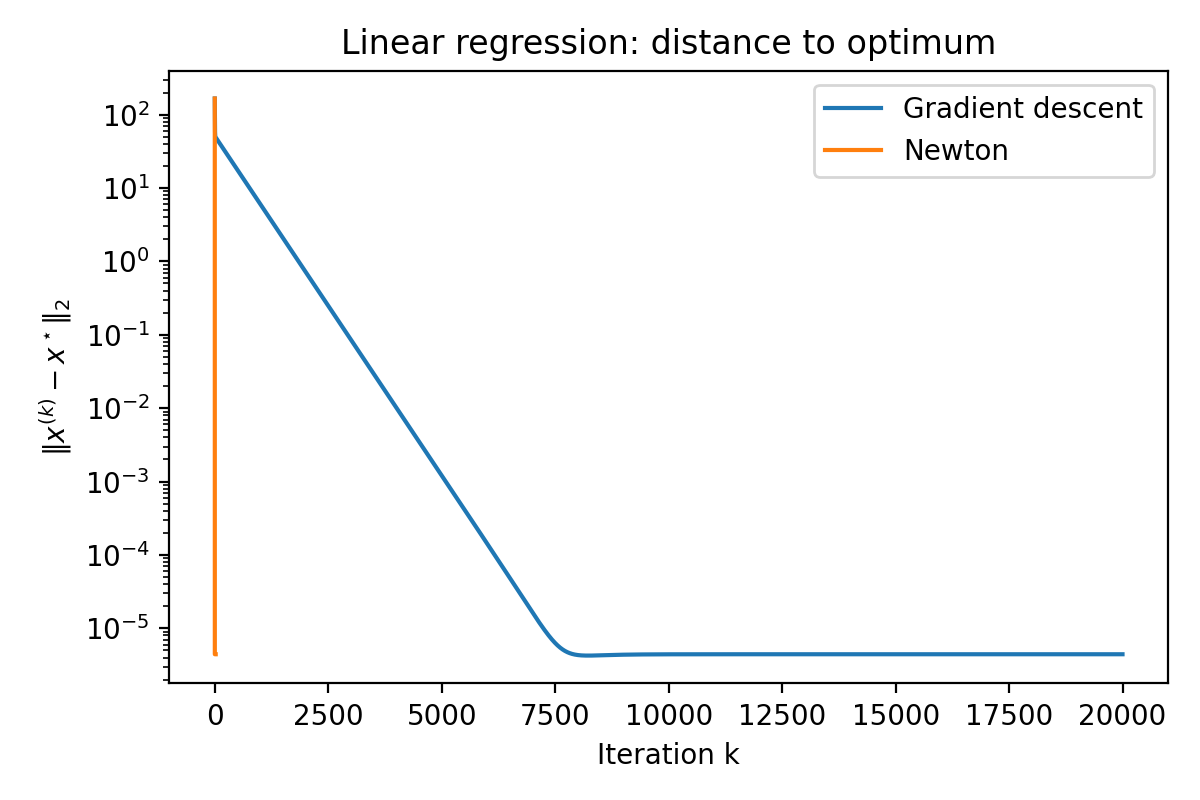
\includegraphics[width=0.48\textwidth]{linear_regression_distance.png}
    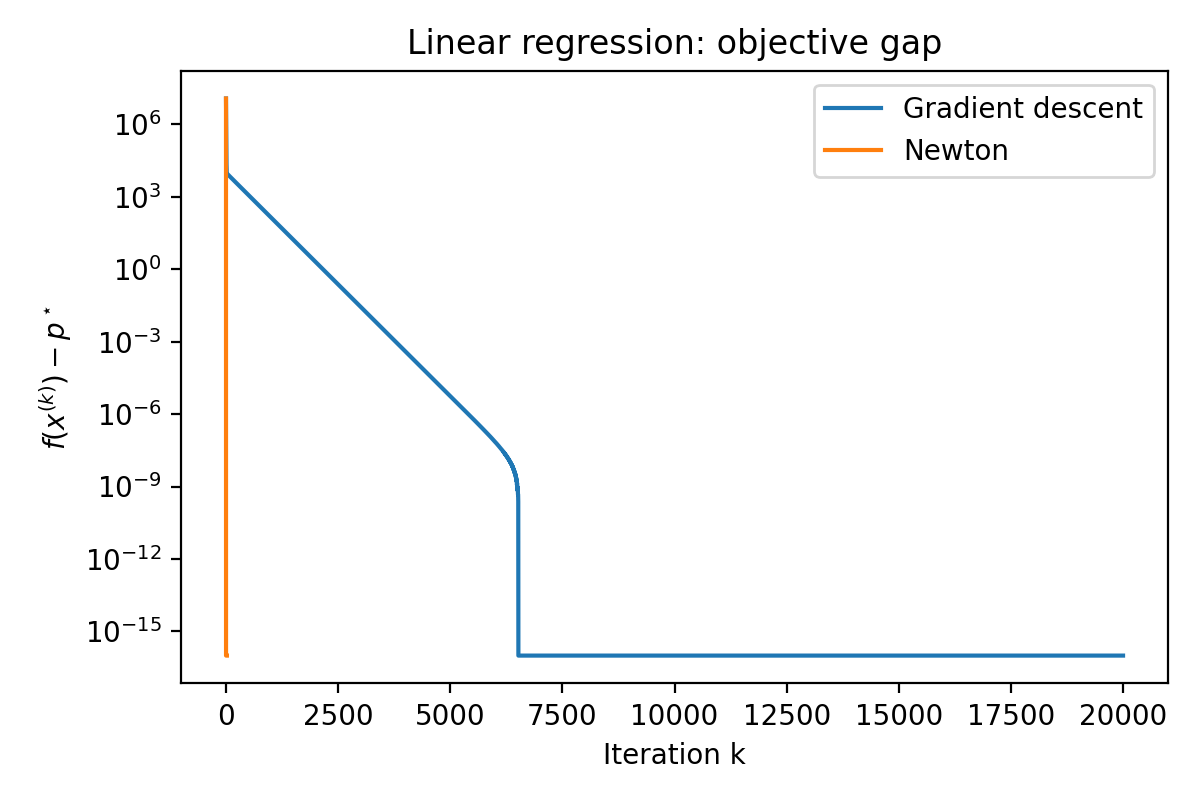
\includegraphics[width=0.48\textwidth]{linear_regression_gap.png}
    \caption{Linear regression: $\|x^{(k)}-x^\star\|_2$ and $f(x^{(k)})-p^\star$ versus iteration count.}
\end{figure}

\begin{figure}[H]
    \centering
    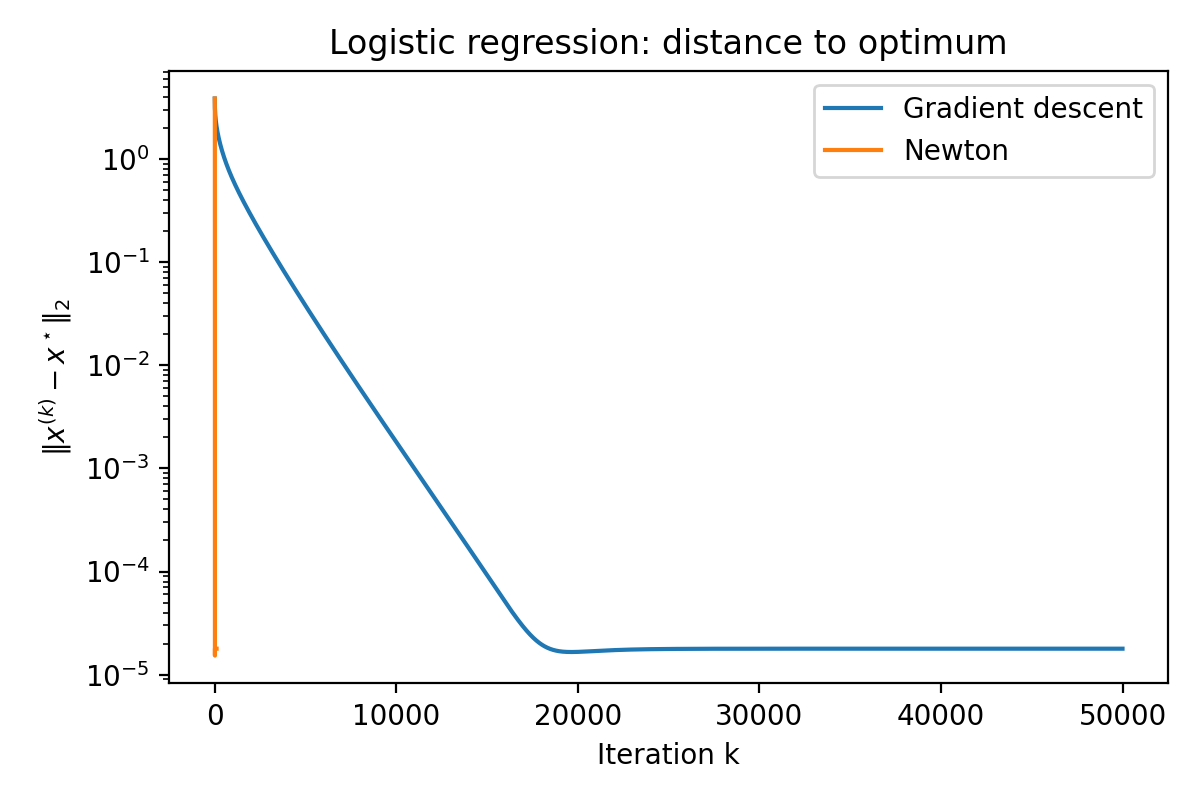
\includegraphics[width=0.48\textwidth]{logistic_regression_distance.png}
    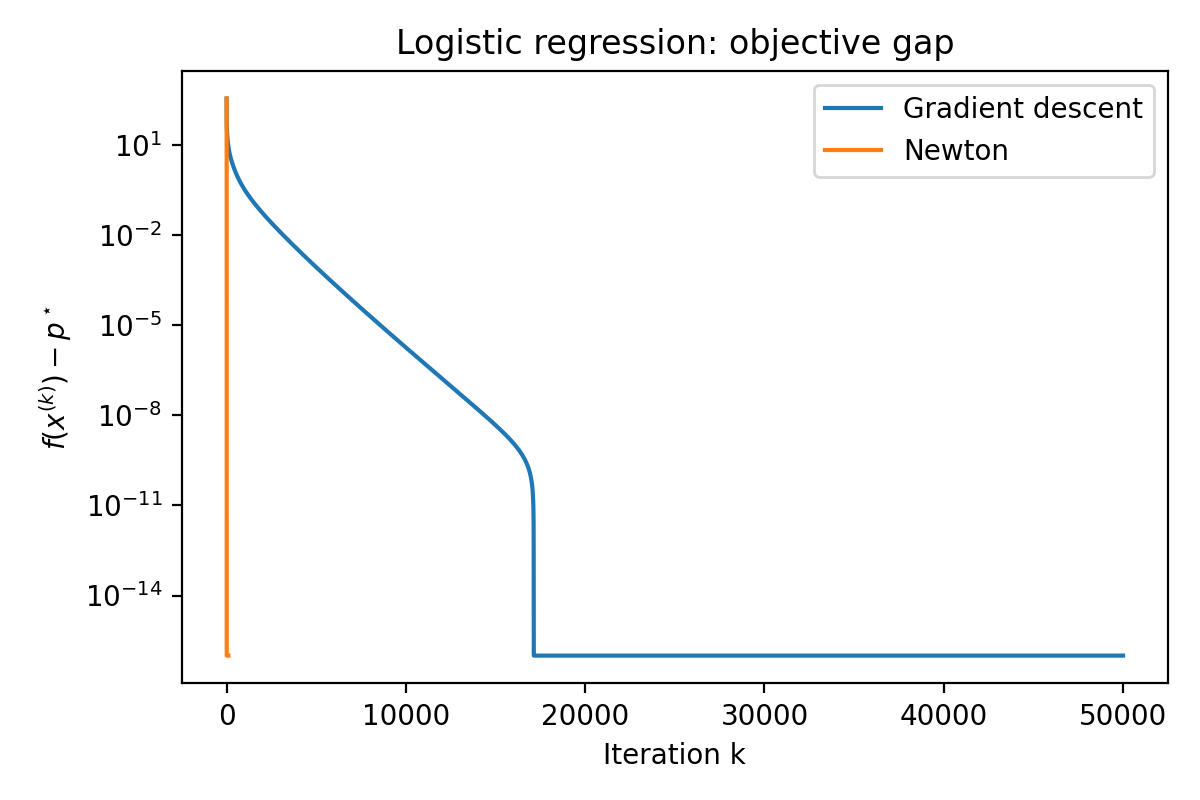
\includegraphics[width=0.48\textwidth]{logistic_regression_gap.png}
    \caption{Logistic regression: $\|x^{(k)}-x^\star\|_2$ and $f(x^{(k)})-p^\star$ versus iteration count.}
\end{figure}

From the plots, gradient descent exhibits linear convergence in both problems, while Newton's method converges dramatically faster. For linear regression, Newton's method essentially reaches the optimum in one step. For logistic regression, Newton's method converges within only a few iterations, while gradient descent requires several thousand iterations.

\item \textbf{Run-time to reach the prescribed RMSE levels.}

We used the criterion
\[
\sqrt{\frac{1}{d}\|x^{(k)}-x^\star\|_2^2}\le \epsilon,
\qquad
\epsilon\in\{10^{-2},10^{-3},10^{-4}\}.
\]

\medskip
\noindent
\textbf{Linear regression:}
\[
\begin{array}{c|ccc}
\text{Method} & \epsilon=10^{-2} & \epsilon=10^{-3} & \epsilon=10^{-4} \\
\hline
\text{Gradient descent} &
(3448,\;0.072157\text{ s}) &
(4529,\;0.093280\text{ s}) &
(5608,\;0.113464\text{ s})
\\
\text{Newton} &
(1,\;0.000165\text{ s}) &
(1,\;0.000165\text{ s}) &
(1,\;0.000165\text{ s})
\end{array}
\]

\medskip
\noindent
\textbf{Logistic regression:}
\[
\begin{array}{c|ccc}
\text{Method} & \epsilon=10^{-2} & \epsilon=10^{-3} & \epsilon=10^{-4} \\
\hline
\text{Gradient descent} &
(4395,\;1.000440\text{ s}) &
(8109,\;1.827914\text{ s}) &
(11981,\;2.820052\text{ s})
\\
\text{Newton} &
(7,\;0.007921\text{ s}) &
(7,\;0.007921\text{ s}) &
(8,\;0.008460\text{ s})
\end{array}
\]

Each pair above is of the form $(\text{iterations}, \text{time})$.

\item \textbf{Explanation of the results.}

The results are fully consistent with the theory.

For linear regression, the objective is a strongly convex quadratic function. Gradient descent with step size $1/L$ converges linearly:
\[
\|x^{(k)}-x^\star\|_2
\le
\left(1-\frac{m}{L}\right)^k
\|x^{(0)}-x^\star\|_2.
\]
Here,
\[
1-\frac{m}{L}
=
1-\frac{7.567685}{3557.402303}
\approx 0.99787.
\]
Thus the convergence is linear but relatively slow compared with Newton's method. Since the Hessian is constant, Newton's method solves the quadratic problem essentially in one iteration, exactly as seen in the plots and timing table.

For logistic regression, after adding $\frac12\gamma\|x\|_2^2$ with $\gamma=1$, the objective becomes globally strongly convex. Gradient descent again converges linearly, but with a worse condition number:
\[
\kappa \approx 1890.308693,
\]
and rate
\[
1-\frac{m}{L}
=
1-\frac{1}{1890.308693}
\approx 0.99947.
\]
Since this number is much closer to $1$, the method needs far more iterations than in linear regression. Newton's method, however, exploits second-order curvature information and therefore converges in only a few steps.

In summary, the experiments confirm the expected theoretical behavior: gradient descent is globally convergent but slow when the condition number is large, whereas Newton's method is much faster, especially for strongly convex problems and particularly for quadratic objectives.

Scripts:
\lstinputlisting[language=Python]{4.py}

\end{enumerate}

\end{solution}

\newpage

\begin{exercise}
Equality constrained entropy maximization. Consider the equality constrained entropy maximization problem
\[
\begin{aligned}
\minimize \quad & f(x) = \sum_{i=1}^n x_i \log x_i \\
\text{subject to} \quad & Ax = b,
\end{aligned}
\]
with $\operatorname{dom} f = \mathbb{R}_{++}^n$ and $A \in \mathbb{R}^{p \times n}$, with $p < n$. (See Exercise 10.9 for some relevant analysis.)

Generate a problem instance with $n = 100$ and $p = 30$ by choosing $A$ randomly (checking that it has full rank), choosing $\hat{x}$ as a random positive vector (e.g., with entries uniformly distributed on $[0,1]$) and then setting $b = A\hat{x}$. (Thus, $\hat{x}$ is feasible.)

Compute the solution of the problem using the following method:

\begin{enumerate}[label=(\alph*)]
    \item \textit{Standard Newton method.} You can use initial point $x^{(0)} = \hat{x}$.
\end{enumerate}
\end{exercise}

\newpage

\begin{solution}
We consider
\[
\begin{aligned}
\minimize \quad & f(x)=\sum_{i=1}^n x_i\log x_i\\
\text{subject to}\quad & Ax=b,
\end{aligned}
\qquad \operatorname{dom}f=\mathbb R_{++}^n.
\]

For this problem,
\[
\nabla f(x)=\log x+\mathbf 1,
\qquad
\nabla^2 f(x)=\operatorname{diag}\!\left(\frac1{x_1},\dots,\frac1{x_n}\right).
\]
Since \(x_i>0\), the Hessian is positive definite, so \(f\) is strictly convex.

Starting from a feasible point \(x^{(0)}=\hat x\) with \(A\hat x=b\), the equality constrained Newton step
\(\Delta x\) is obtained from
\[
\begin{aligned}
\minimize_{\Delta x}\quad
& \nabla f(x)^T\Delta x+\frac12 \Delta x^T\nabla^2 f(x)\Delta x\\
\text{subject to}\quad
& A\Delta x=0.
\end{aligned}
\]
Its KKT system is
\[
\begin{bmatrix}
\nabla^2 f(x) & A^T\\
A & 0
\end{bmatrix}
\begin{bmatrix}
\Delta x\\
w
\end{bmatrix}
=
\begin{bmatrix}
-\nabla f(x)\\
0
\end{bmatrix}.
\]
Thus, for the entropy objective,
\[
\begin{bmatrix}
\operatorname{diag}(1/x) & A^T\\
A & 0
\end{bmatrix}
\begin{bmatrix}
\Delta x\\
w
\end{bmatrix}
=
\begin{bmatrix}
-(\log x+\mathbf 1)\\
0
\end{bmatrix}.
\]

Using \(\operatorname{diag}(1/x)^{-1}=\operatorname{diag}(x)\), we can write
\[
\Delta x=-\operatorname{diag}(x)\bigl(\log x+\mathbf 1+A^T w\bigr),
\]
where \(w\) solves
\[
A\operatorname{diag}(x)A^T\,w
=
-A\operatorname{diag}(x)(\log x+\mathbf 1).
\]

The update is
\[
x^+=x+t\Delta x,
\]
where \(t\) is chosen by backtracking line search to ensure \(x^+\in\mathbb R_{++}^n\) and sufficient decrease. Since \(A\Delta x=0\), all iterates remain feasible:
\[
A(x+t\Delta x)=Ax+tA\Delta x=b.
\]

We generated a random instance with \(n=100\) and \(p=30\), choosing \(A\in\mathbb R^{30\times 100}\) randomly and verifying that it has full rank, then choosing a random positive vector \(\hat x\) and setting
\[
b=A\hat x.
\]
Hence \(\hat x\) is feasible and was used as the initial point.

For the generated instance, the numerical results were:
\[
\operatorname{rank}(A)=30,
\qquad
\text{iterations}=8,
\]
\[
f(x^{(0)})=-26.818061118030787,
\qquad
f(x^\star)=-33.12710780279478.
\]
The final feasibility residual and stationarity residual were
\[
\|Ax^\star-b\|_2=2.7330716731741607\times 10^{-14},
\]
\[
\|\nabla f(x^\star)+A^T\nu^\star\|_\infty
=7.257538459093382\times 10^{-10}.
\]
Thus the method converged to high accuracy.

The iteration history is:
\[
\begin{array}{c|c|c|c}
k & f(x^{(k)}) & \lambda(x^{(k)})^2/2 & \|Ax^{(k)}-b\|_2\\
\hline
0 & -26.8180611180 & 7.1245633754 & 0.000\times 10^0\\
1 & -32.4582941311 & 4.3215733648\times 10^{-1} & 1.454\times 10^{-14}\\
2 & -32.9507074296 & 9.9299435643\times 10^{-2} & 1.912\times 10^{-14}\\
3 & -33.0780393631 & 3.9056131947\times 10^{-2} & 2.269\times 10^{-14}\\
4 & -33.1235739220 & 3.3735634962\times 10^{-3} & 1.630\times 10^{-14}\\
5 & -33.1270925679 & 1.5192329576\times 10^{-5} & 2.014\times 10^{-14}\\
6 & -33.1271078025 & 2.6608417102\times 10^{-10} & 2.611\times 10^{-14}\\
7 & -33.1271078028 & 1.2905301912\times 10^{-15} & 2.733\times 10^{-14}
\end{array}
\]

Therefore, the standard Newton method solves this equality constrained entropy minimization problem very efficiently.

Scripts:
\lstinputlisting[language=Python]{5.py}
\end{solution}

\newpage

\begin{exercise}
Develop code for solving an LP in the following standard form using the barrier method:
\[
\begin{aligned}
\minimize \quad & c^T x \\
\text{subject to} \quad & Ax=b,\; x \succeq 0.
\end{aligned}
\]

\begin{enumerate}[label=(\alph*)]
    \item Illustrate the progress of the algorithm in a properly chosen random instance $(n=100, m=500$, where $A \in \mathbb{R}^{n\times m})$; additionally, compare with CVXPY and interpret your findings.

    \item For fixed $n$, solve multiple instances by varying $m \in [10,1000]$ to report the number of Newton steps needed. Compare with the expected relation (11.29) in the reference book and interpret your results.
    
    \textit{[}
\[
\begin{aligned}
N
&\le
\left\lceil
\frac{\log\!\bigl(m/(t^{(0)}\epsilon)\bigr)}{\log \mu}
\right\rceil
\left(
\frac{m(\mu-1-\log\mu)}{\gamma}+c
\right) \\
&\le
\left\lceil
\sqrt{m}\,
\frac{\log\!\bigl(m/(t^{(0)}\epsilon)\bigr)}{\log 2}
\right\rceil
\left(
\frac{1}{2\gamma}+c
\right) \\
&=
\left\lceil
\sqrt{m}\,\log_2\!\bigl(m/(t^{(0)}\epsilon)\bigr)
\right\rceil
\left(
\frac{1}{2\gamma}+c
\right) \\
&\le c_1 + c_2\sqrt{m},
\end{aligned}
\tag{11.29}
\]
where
\[
c_1=\frac{1}{2\gamma}+c,
\qquad
c_2=\log_2\!\bigl(m/(t^{(0)}\epsilon)\bigr)\left(\frac{1}{2\gamma}+c\right).
\]
\textit{]}
\end{enumerate}
\end{exercise}

\newpage

\begin{solution}
We solve
\[
\begin{aligned}
\minimize \quad & c^T x\\
\text{subject to}\quad & Ax=b,\quad x \succeq 0
\end{aligned}
\]
by the logarithmic barrier method. For a barrier parameter $t>0$, consider
\[
\begin{aligned}
\minimize \quad & \phi_t(x):= t\,c^T x-\sum_{i=1}^m \log x_i\\
\text{subject to}\quad & Ax=b.
\end{aligned}
\]
The gradient and Hessian are
\[
\nabla \phi_t(x)= t c-\frac{1}{x},
\qquad
\nabla^2 \phi_t(x)=\operatorname{diag}\!\left(\frac{1}{x_1^2},\dots,\frac{1}{x_m^2}\right).
\]
Hence the equality-constrained Newton system is
\[
\begin{bmatrix}
\nabla^2 \phi_t(x) & A^T\\
A & 0
\end{bmatrix}
\begin{bmatrix}
\Delta x\\
w
\end{bmatrix}
=
-
\begin{bmatrix}
\nabla \phi_t(x)\\
0
\end{bmatrix}.
\]
Since the Hessian is diagonal, we solve the reduced Schur complement system
\[
A H^{-1} A^T w = - A H^{-1} g,
\]
where
\[
g = t c-\frac{1}{x},
\qquad
H^{-1}=\operatorname{diag}(x_1^2,\dots,x_m^2),
\]
and then recover
\[
\Delta x = -H^{-1}(g+A^T w).
\]
A backtracking line search is used to keep $x+\alpha \Delta x \succ 0$, and the outer barrier update is
\[
t \leftarrow \mu t,
\]
with stopping rule
\[
\frac{m}{t}<\varepsilon.
\]

\paragraph{(a) Random instance with $n=100$, $m=500$.}
We generated a strictly feasible random instance by first sampling a full-row-rank matrix
$A\in\mathbb{R}^{100\times 500}$, then choosing $x^{(0)} \succ 0$ and setting
\[
b=Ax^{(0)}.
\]
Thus $x^{(0)}$ is a strictly feasible initial point. We used the parameters
\[
\mu=10,\qquad \varepsilon=10^{-8},
\qquad \text{Newton tolerance }=10^{-8}.
\]

The barrier method produced the following summary:
\[
\begin{array}{|c|c|}
\hline
\text{runtime} & 3.899693489075\times 10^{-2}\ \text{s}\\
\hline
\text{objective value} & -2.612142768173\times 10^2\\
\hline
\text{total Newton steps} & 68\\
\hline
\text{outer iterations} & 12\\
\hline
\|Ax-b\|_2 & 1.520264944125\times 10^{-5}\\
\hline
\min_i x_i & 2.358572704445\times 10^{-8}\\
\hline
\end{array}
\]

To illustrate the progress of the algorithm, the outer iteration history is shown below:
\[
\begin{array}{|c|c|c|c|c|c|c|}
\hline
k & t & c^T x^{(k)} & m/t & \text{Newton steps} & \|Ax^{(k)}-b\|_2 & \min_i x_i^{(k)}\\
\hline
0 & 10^0   & 1.154273\times 10^2   & 5.0\times 10^2 & 10 & 1.245937\times 10^{-11} & 5.172649\times 10^{-1}\\
\hline
1 & 10^1   & -2.228975\times 10^2  & 5.0\times 10^1 & 12 & 9.512006\times 10^{-11} & 3.853261\times 10^{-2}\\
\hline
2 & 10^2   & -2.572903\times 10^2  & 5.0\times 10^0 & 12 & 1.500768\times 10^{-9}  & 3.294768\times 10^{-3}\\
\hline
3 & 10^3   & -2.608136\times 10^2  & 5.0\times 10^{-1} & 14 & 1.745518\times 10^{-8}  & 3.244546\times 10^{-4}\\
\hline
4 & 10^4   & -2.611742\times 10^2  & 5.0\times 10^{-2} & 9  & 1.397381\times 10^{-7}  & 3.242947\times 10^{-5}\\
\hline
5 & 10^5   & -2.612103\times 10^2  & 5.0\times 10^{-3} & 7  & 9.703330\times 10^{-7}  & 3.252327\times 10^{-6}\\
\hline
6 & 10^6   & -2.612139\times 10^2  & 5.0\times 10^{-4} & 2  & 2.014618\times 10^{-6}  & 3.451718\times 10^{-7}\\
\hline
7 & 10^7   & -2.612143\times 10^2  & 5.0\times 10^{-5} & 2  & 1.520265\times 10^{-5}  & 2.358573\times 10^{-8}\\
\hline
8 & 10^8   & -2.612143\times 10^2  & 5.0\times 10^{-6} & 0  & 1.520265\times 10^{-5}  & 2.358573\times 10^{-8}\\
\hline
9 & 10^9   & -2.612143\times 10^2  & 5.0\times 10^{-7} & 0  & 1.520265\times 10^{-5}  & 2.358573\times 10^{-8}\\
\hline
10 & 10^{10} & -2.612143\times 10^2 & 5.0\times 10^{-8} & 0  & 1.520265\times 10^{-5}  & 2.358573\times 10^{-8}\\
\hline
11 & 10^{11} & -2.612143\times 10^2 & 5.0\times 10^{-9} & 0  & 1.520265\times 10^{-5}  & 2.358573\times 10^{-8}\\
\hline
\end{array}
\]

We compare the result with CVXPY:
\[
\begin{array}{|c|c|c|c|c|c|}
\hline
\text{solver} & \text{status} & \text{time (s)} & \text{objective} & \|Ax-b\|_2 & \text{obj.\ diff.\ vs barrier}\\
\hline
\texttt{CLARABEL} & \texttt{optimal} & 2.548163\times 10^{-1}
& -2.612143\times 10^2 & 2.199587\times 10^{-13} & 3.709935\times 10^{-5}\\
\hline
\texttt{SCS} & \texttt{optimal} & 1.479883\times 10^{-1}
& -2.612157\times 10^2 & 9.885638\times 10^{-6} & 1.376633\times 10^{-3}\\
\hline
\end{array}
\]

\textbf{Interpretation.}
The objective value decreases rapidly and stabilizes near
\[
p^\star \approx -2.612143\times 10^2.
\]
The duality-gap estimate $m/t$ decreases by a factor of $10$ at each outer iteration, exactly as expected. The barrier solution is very close to the CVXPY solution, especially to \texttt{CLARABEL}, whose objective differs only by about $3.7\times 10^{-5}$. Thus the implementation is correct.

However, from outer iterations $8$--$11$, the Newton step count becomes zero and the equality residual remains around $1.5\times 10^{-5}$. This indicates numerical stagnation: once $t$ becomes very large, the barrier subproblem becomes badly conditioned, so further increasing $t$ no longer improves the iterate significantly. In practice, the useful convergence has already occurred by about $t=10^6$ or $10^7$.

\paragraph{(b) Scaling with respect to $m$.}
To study the dependence on $m$, we fixed $n=5$ and varied
\[
m\in\{10,20,50,100,200,400,600,800,1000\}.
\]
We chose
\[
\mu = 1+\frac{1}{\sqrt{m}},
\]
which is closer to the short-step schedule underlying the theoretical bound (11.29). For each $m$, we solved $3$ random instances and recorded the total number of Newton steps. The results are:

\[
\begin{array}{|c|c|c|c|c|}
\hline
m & \mu & \text{mean total Newton steps} & \text{std} & \text{mean outer iterations}\\
\hline
10   & 1.316228 & 50.000000  & 3.265986 & 18.0\\
\hline
20   & 1.223607 & 59.666667  & 1.699673 & 28.0\\
\hline
50   & 1.141421 & 98.666667  & 0.471405 & 48.0\\
\hline
100  & 1.100000 & 153.666667 & 1.247219 & 74.0\\
\hline
200  & 1.070711 & 233.000000 & 0.000000 & 113.0\\
\hline
400  & 1.050000 & 349.000000 & 0.000000 & 171.0\\
\hline
600  & 1.040825 & 445.000000 & 0.000000 & 219.0\\
\hline
800  & 1.035355 & 527.000000 & 0.000000 & 260.0\\
\hline
1000 & 1.031623 & 601.000000 & 0.000000 & 297.0\\
\hline
\end{array}
\]

A least-squares fit against $\sqrt{m}$ gives
\[
N \approx 19.649522\,\sqrt{m}-33.087274,
\qquad
R^2 = 0.996964.
\]
A fit against $\sqrt{m}\log_2 m$ gives
\[
N \approx 1.826148\,\sqrt{m}\log_2 m + 29.863497,
\qquad
R^2 = 0.999645.
\]

\textbf{Interpretation.}
These experiments are consistent with the theoretical relation (11.29). Indeed, the book predicts
\[
N = O\!\bigl(\sqrt{m}\log(m/(t^{(0)}\epsilon))\bigr).
\]
Over the finite range $10\le m\le 1000$, the logarithmic factor varies slowly, so the total step count already looks nearly linear in $\sqrt{m}$. The better fit with $\sqrt{m}\log_2 m$ confirms that the observed behavior is even closer to the theoretical upper bound than a pure $\sqrt{m}$ law.

Therefore, the numerical experiment supports the conclusion that the Newton complexity of the barrier method grows roughly like $\sqrt{m}$ up to a slowly varying logarithmic factor, in agreement with the theory.

Scripts:
\lstinputlisting[language=Python]{6.py}
\end{solution}
	
\end{document}
